\documentclass[10pt]{article}

\usepackage[a4paper,margin=0.55in]{geometry}
\usepackage{graphicx}
\usepackage{booktabs}
\usepackage{tabularx}
\usepackage{xcolor}
\usepackage{array}

\setlength{\parindent}{0pt}
\setlength{\parskip}{0.35em}
\renewcommand{\arraystretch}{1.08}
\definecolor{muted}{RGB}{75,85,99}

\title{\vspace{-1.6em}Quick progress update}
\author{Samuel Barber}
\date{15 May 2026}

\begin{document}
\maketitle
\vspace{-1.4em}

\section*{Dataset: paired and pixel-aligned}

\textbf{Collection since last update.} Since the last update I have cycled for more than 20 hours around London collecting paired street-level RGB/NIR data. The capture device was mounted to my bag so it could record real scenes continuously while moving.

\begin{center}
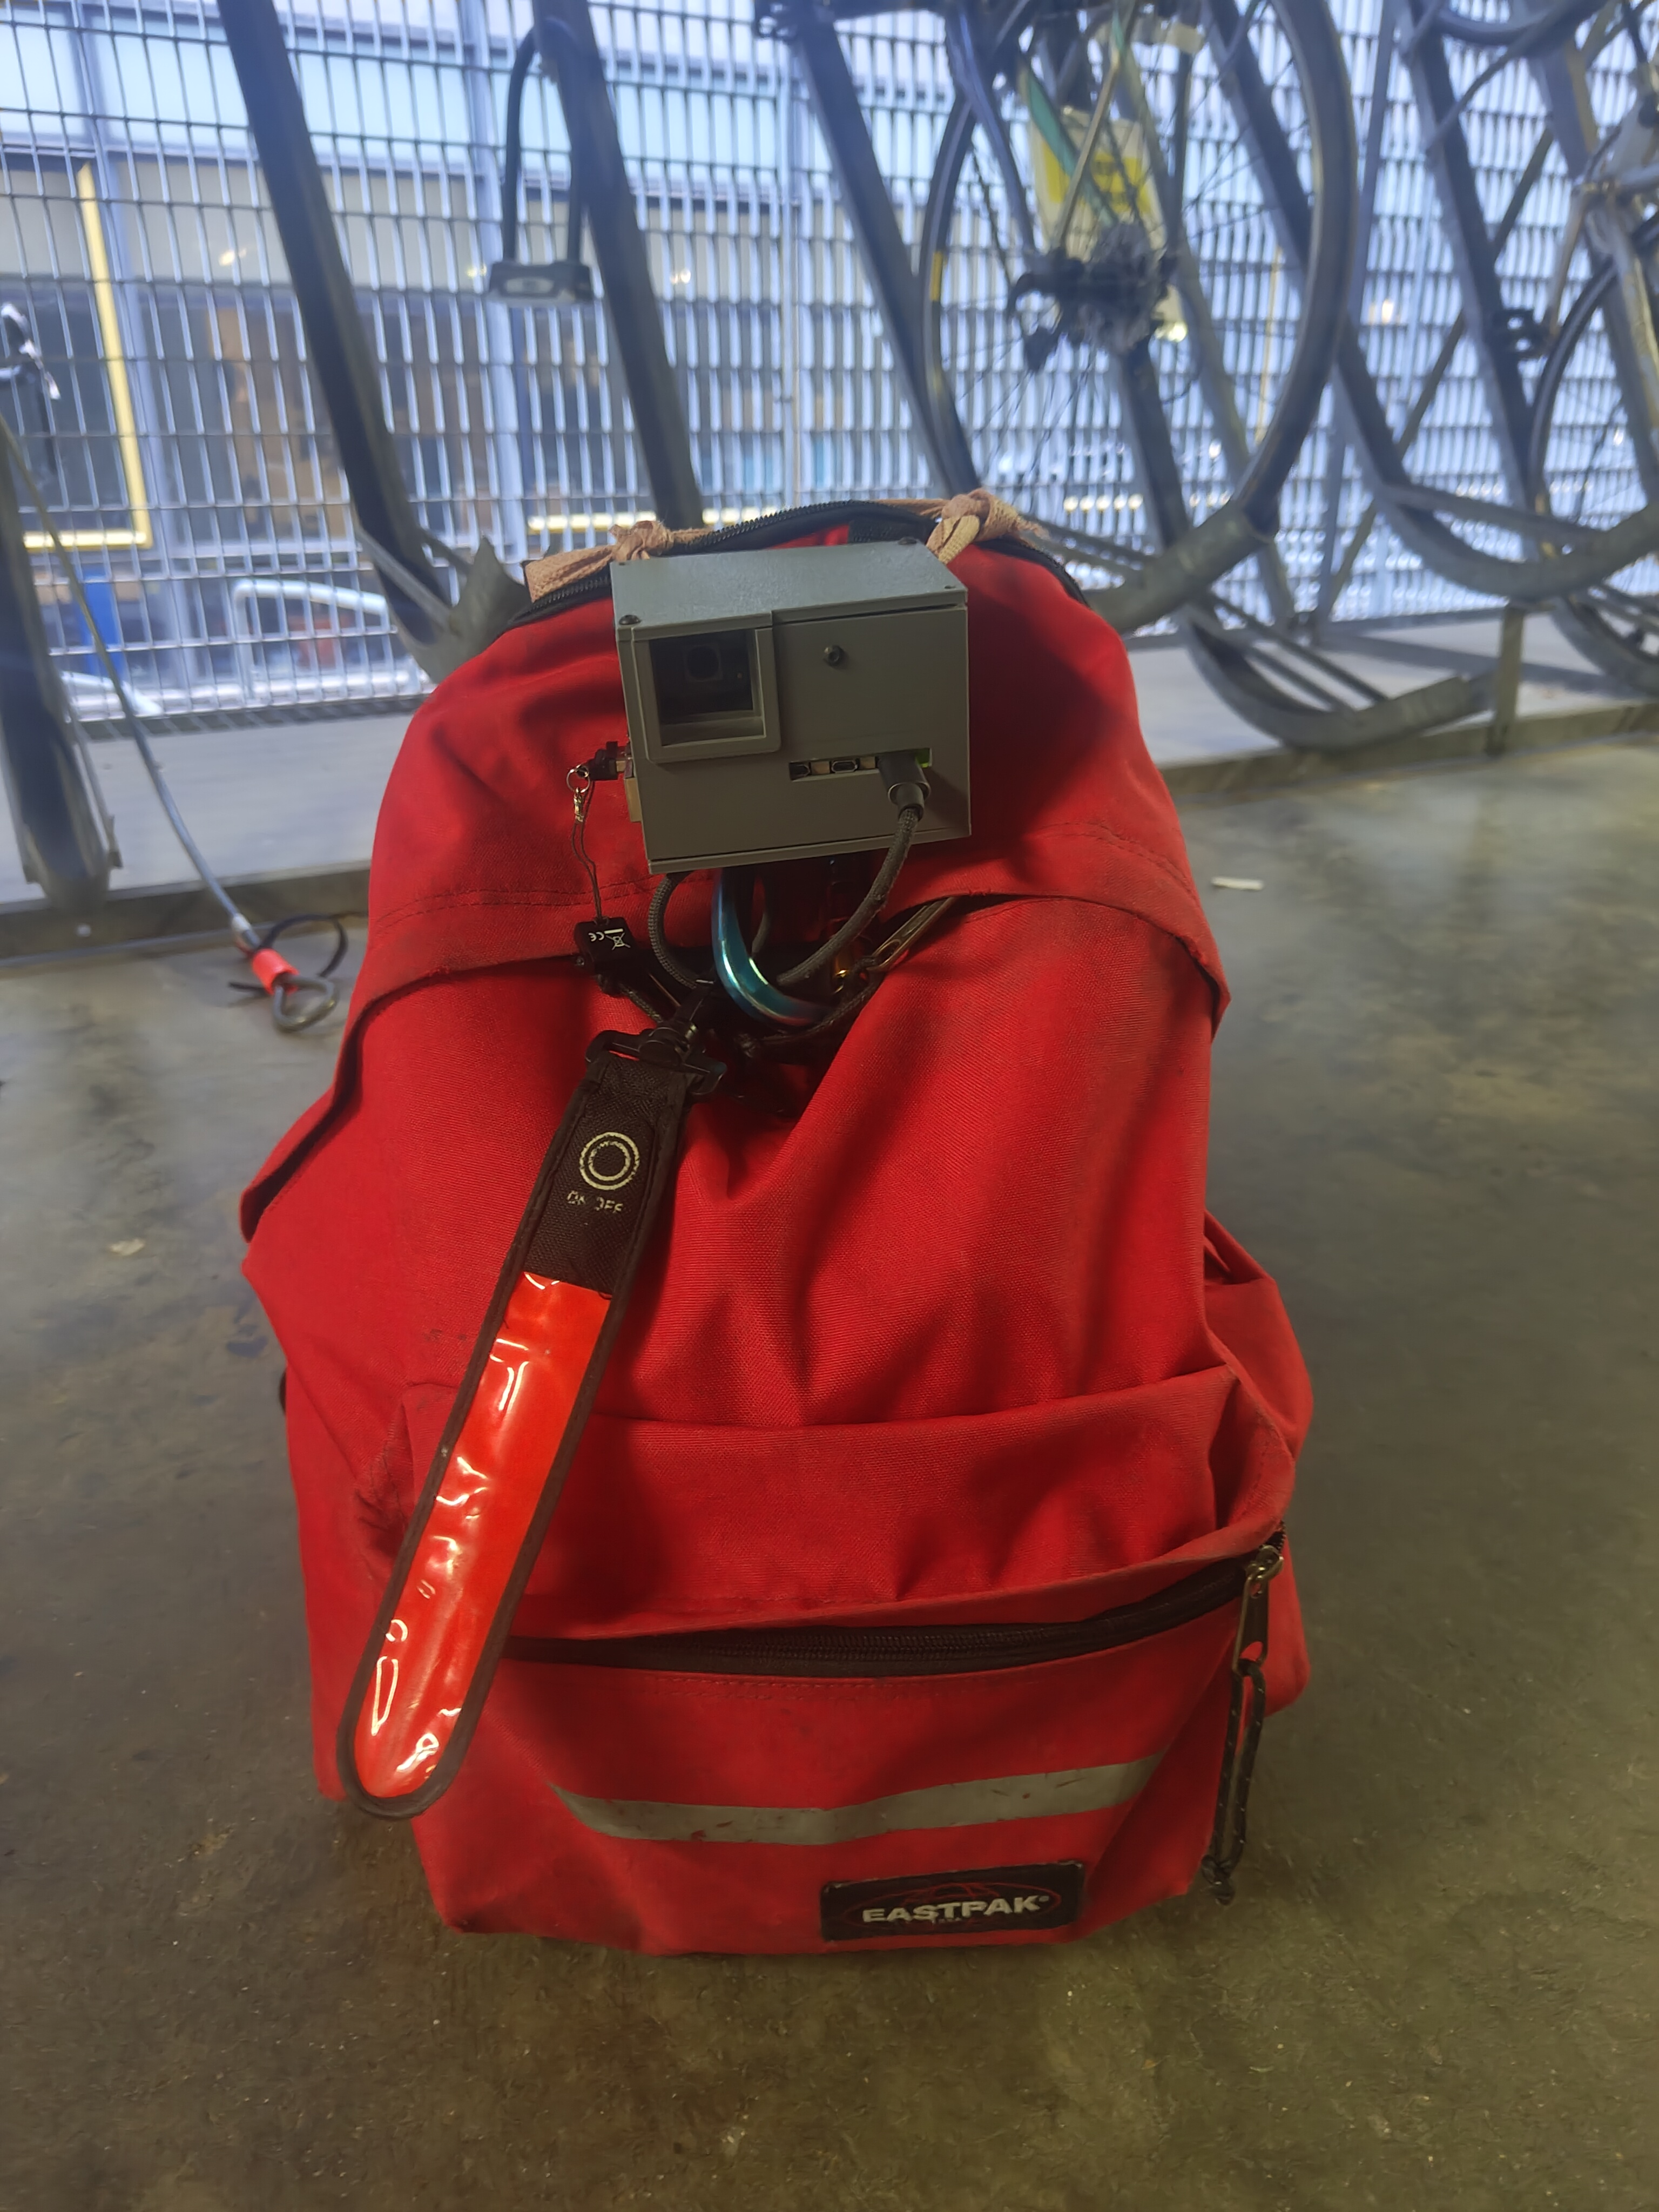
\includegraphics[height=0.38\textheight]{figures/IMG_20260504_194300907.jpg}
\end{center}

\textbf{Current usable data:} 12,536 paired RGB/NIR images after blur filtering and SIFT/RANSAC alignment. Split: 10,028 train / 1,253 validation / 1,255 test.

\begin{center}
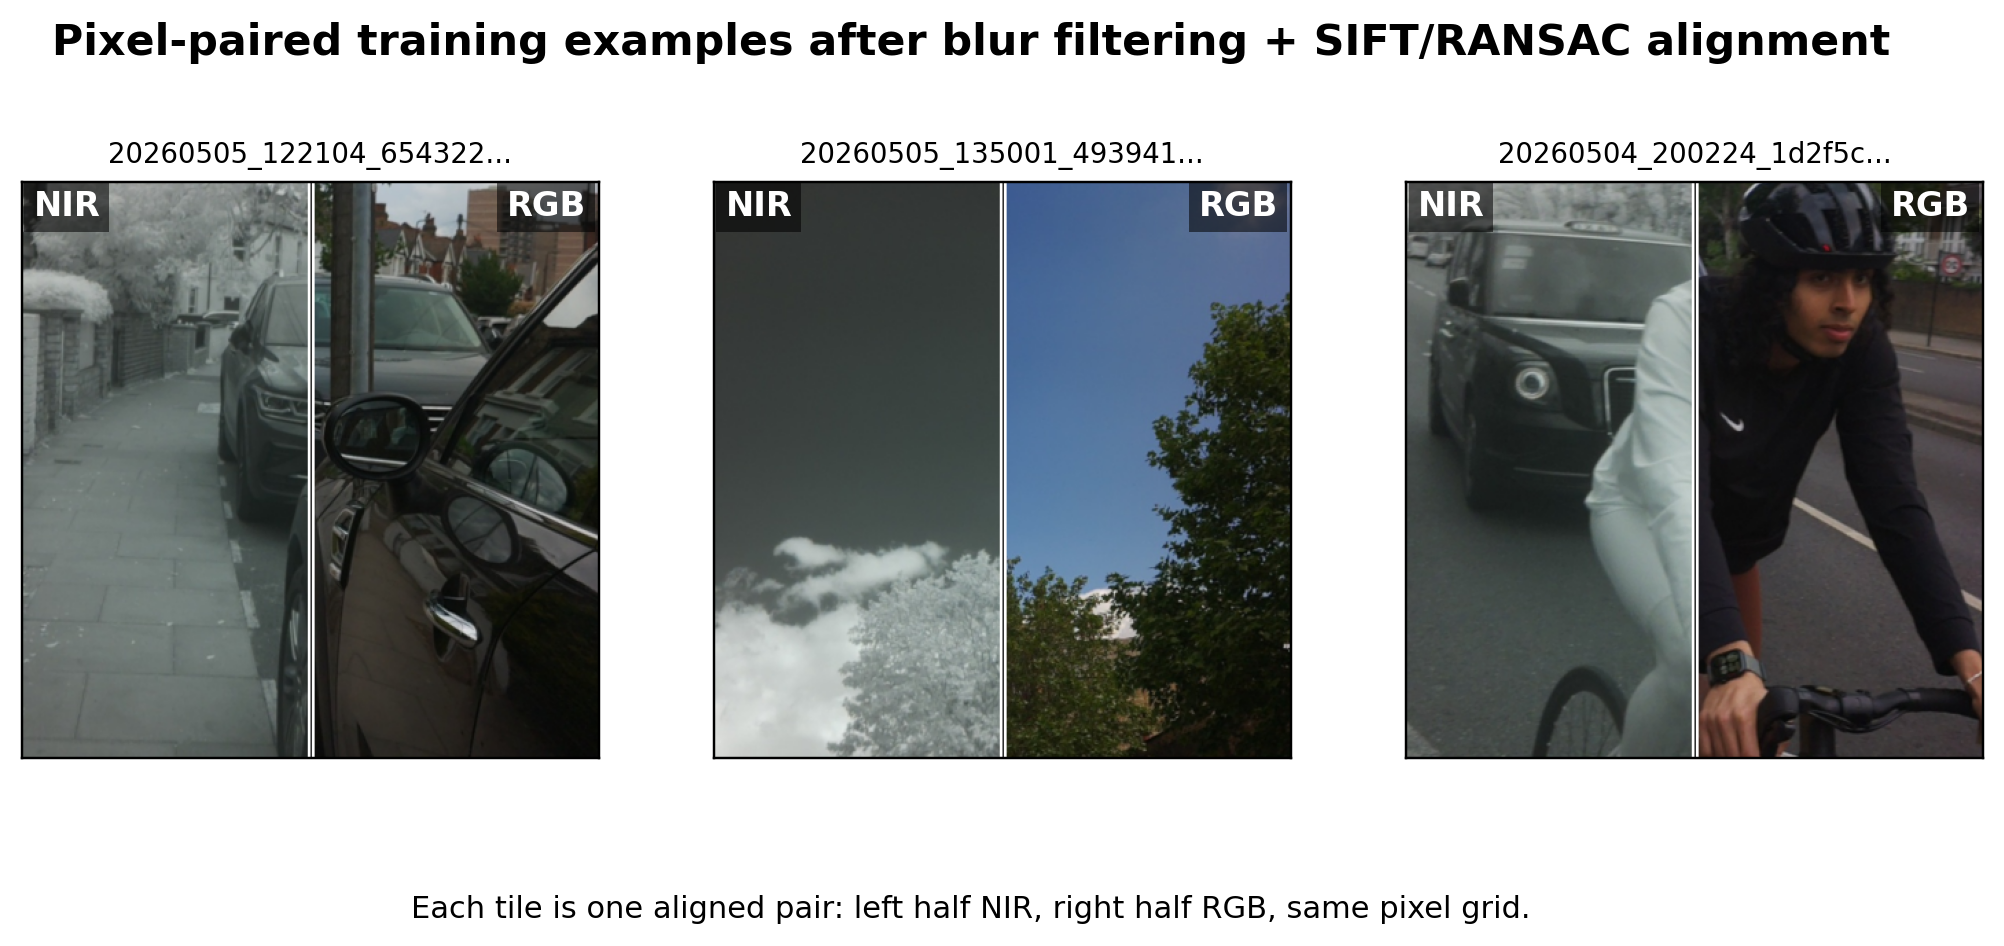
\includegraphics[width=0.94\textwidth]{figures/dataset_pixel_pairs.png}
\end{center}

\newpage
\section*{Teacher model and downstream performance}

\begin{center}
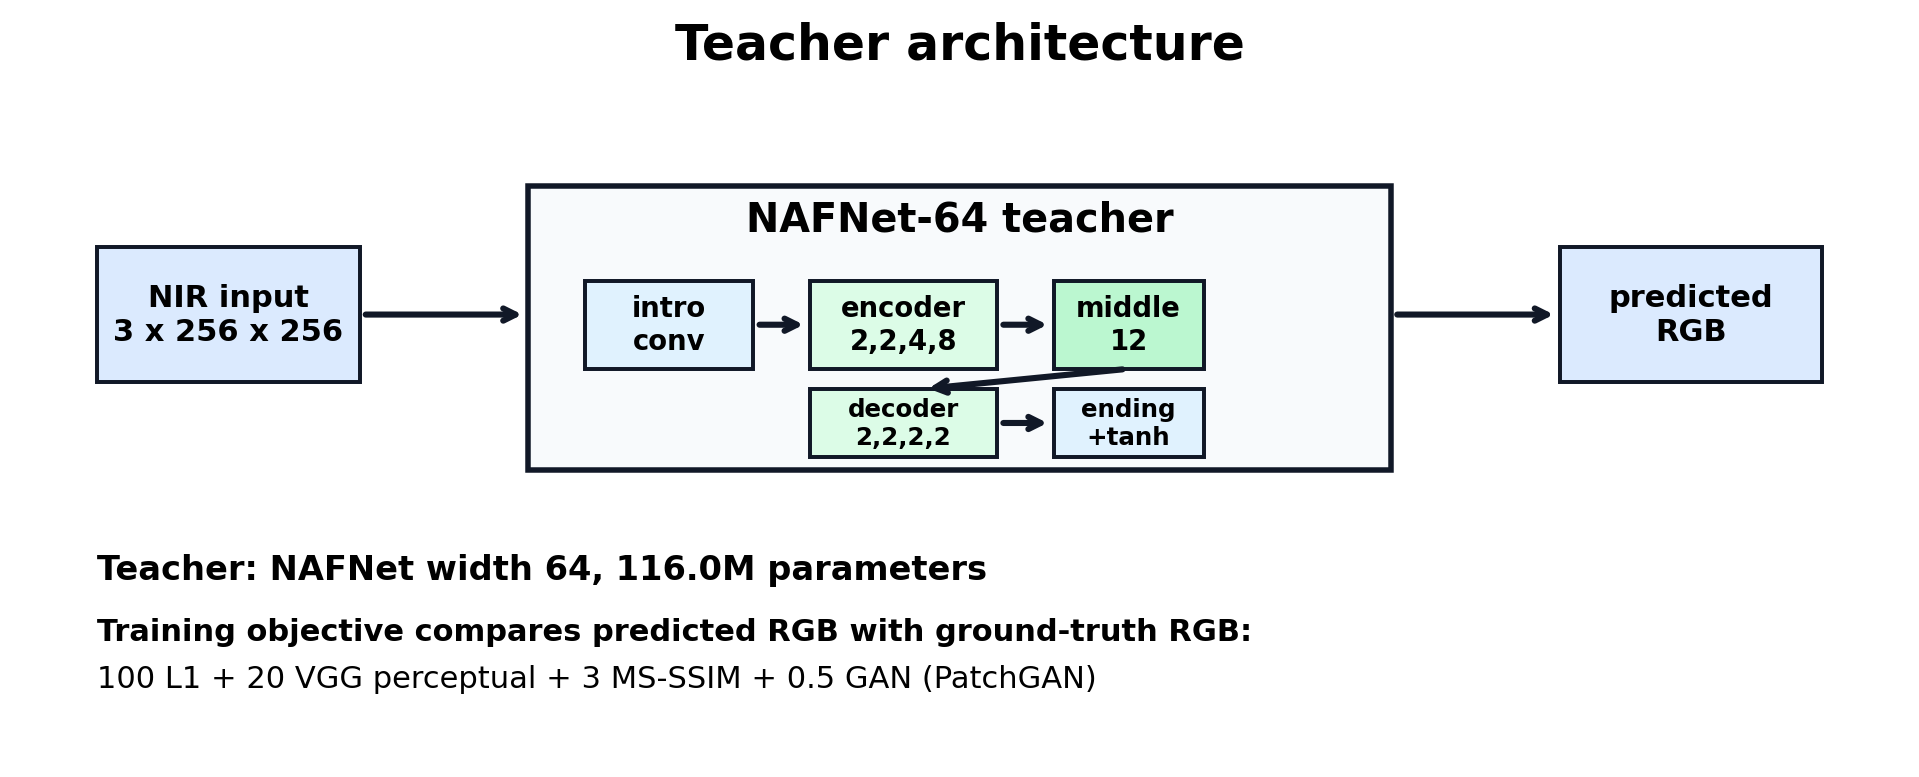
\includegraphics[width=0.92\textwidth]{figures/baseline_architecture.png}
\end{center}

I am using NAFNet for the teacher because it has worked best out of the architectures I have tried so far, and it looks like a reasonable architecture to distil into a smaller edge model later. NAFNet itself is not new; it is normally used for image restoration/reconstruction. As far as I can tell, it has not previously been used directly for NIR/IR/thermal to RGB image conversion. The useful part of this work is the paired dataset, applying NAFNet to this modality conversion problem, and testing whether it actually helps downstream RGB-trained models.

\vspace{-0.3em}
\begin{center}
\scriptsize
\begin{tabular}{llrrrc}
\toprule
Model & Metric vs RGB & raw NIR & translated RGB & gap closure & result \\
\midrule
MediaPipe hands & detection match & 0.965 & 0.965 & +0.0\% & flat \\
MediaPipe selfie & mask IoU & 0.887 & 0.789 & -86.9\% & worse \\
YOLO & matched IoU & 0.778 & 0.797 & +8.6\% & better \\
DeepLabV3 & mIoU & 0.789 & 0.843 & +25.4\% & better \\
Mask R-CNN & matched IoU & 0.761 & 0.784 & +9.3\% & better \\
ResNet50 & top-1 agreement & 0.295 & 0.530 & +33.3\% & better \\
MiDaS & depth rank corr. & 0.863 & 0.954 & +66.2\% & better \\
\bottomrule
\end{tabular}
\end{center}

The basic teacher model already improves most tested RGB-pretrained ML models versus raw NIR, especially MiDaS, ResNet50, DeepLabV3, YOLO, and Mask R-CNN. I am now looking at ways to make that gain bigger and less task-specific. It still does not fix MediaPipe-style skin/landmark tasks.

\begin{center}
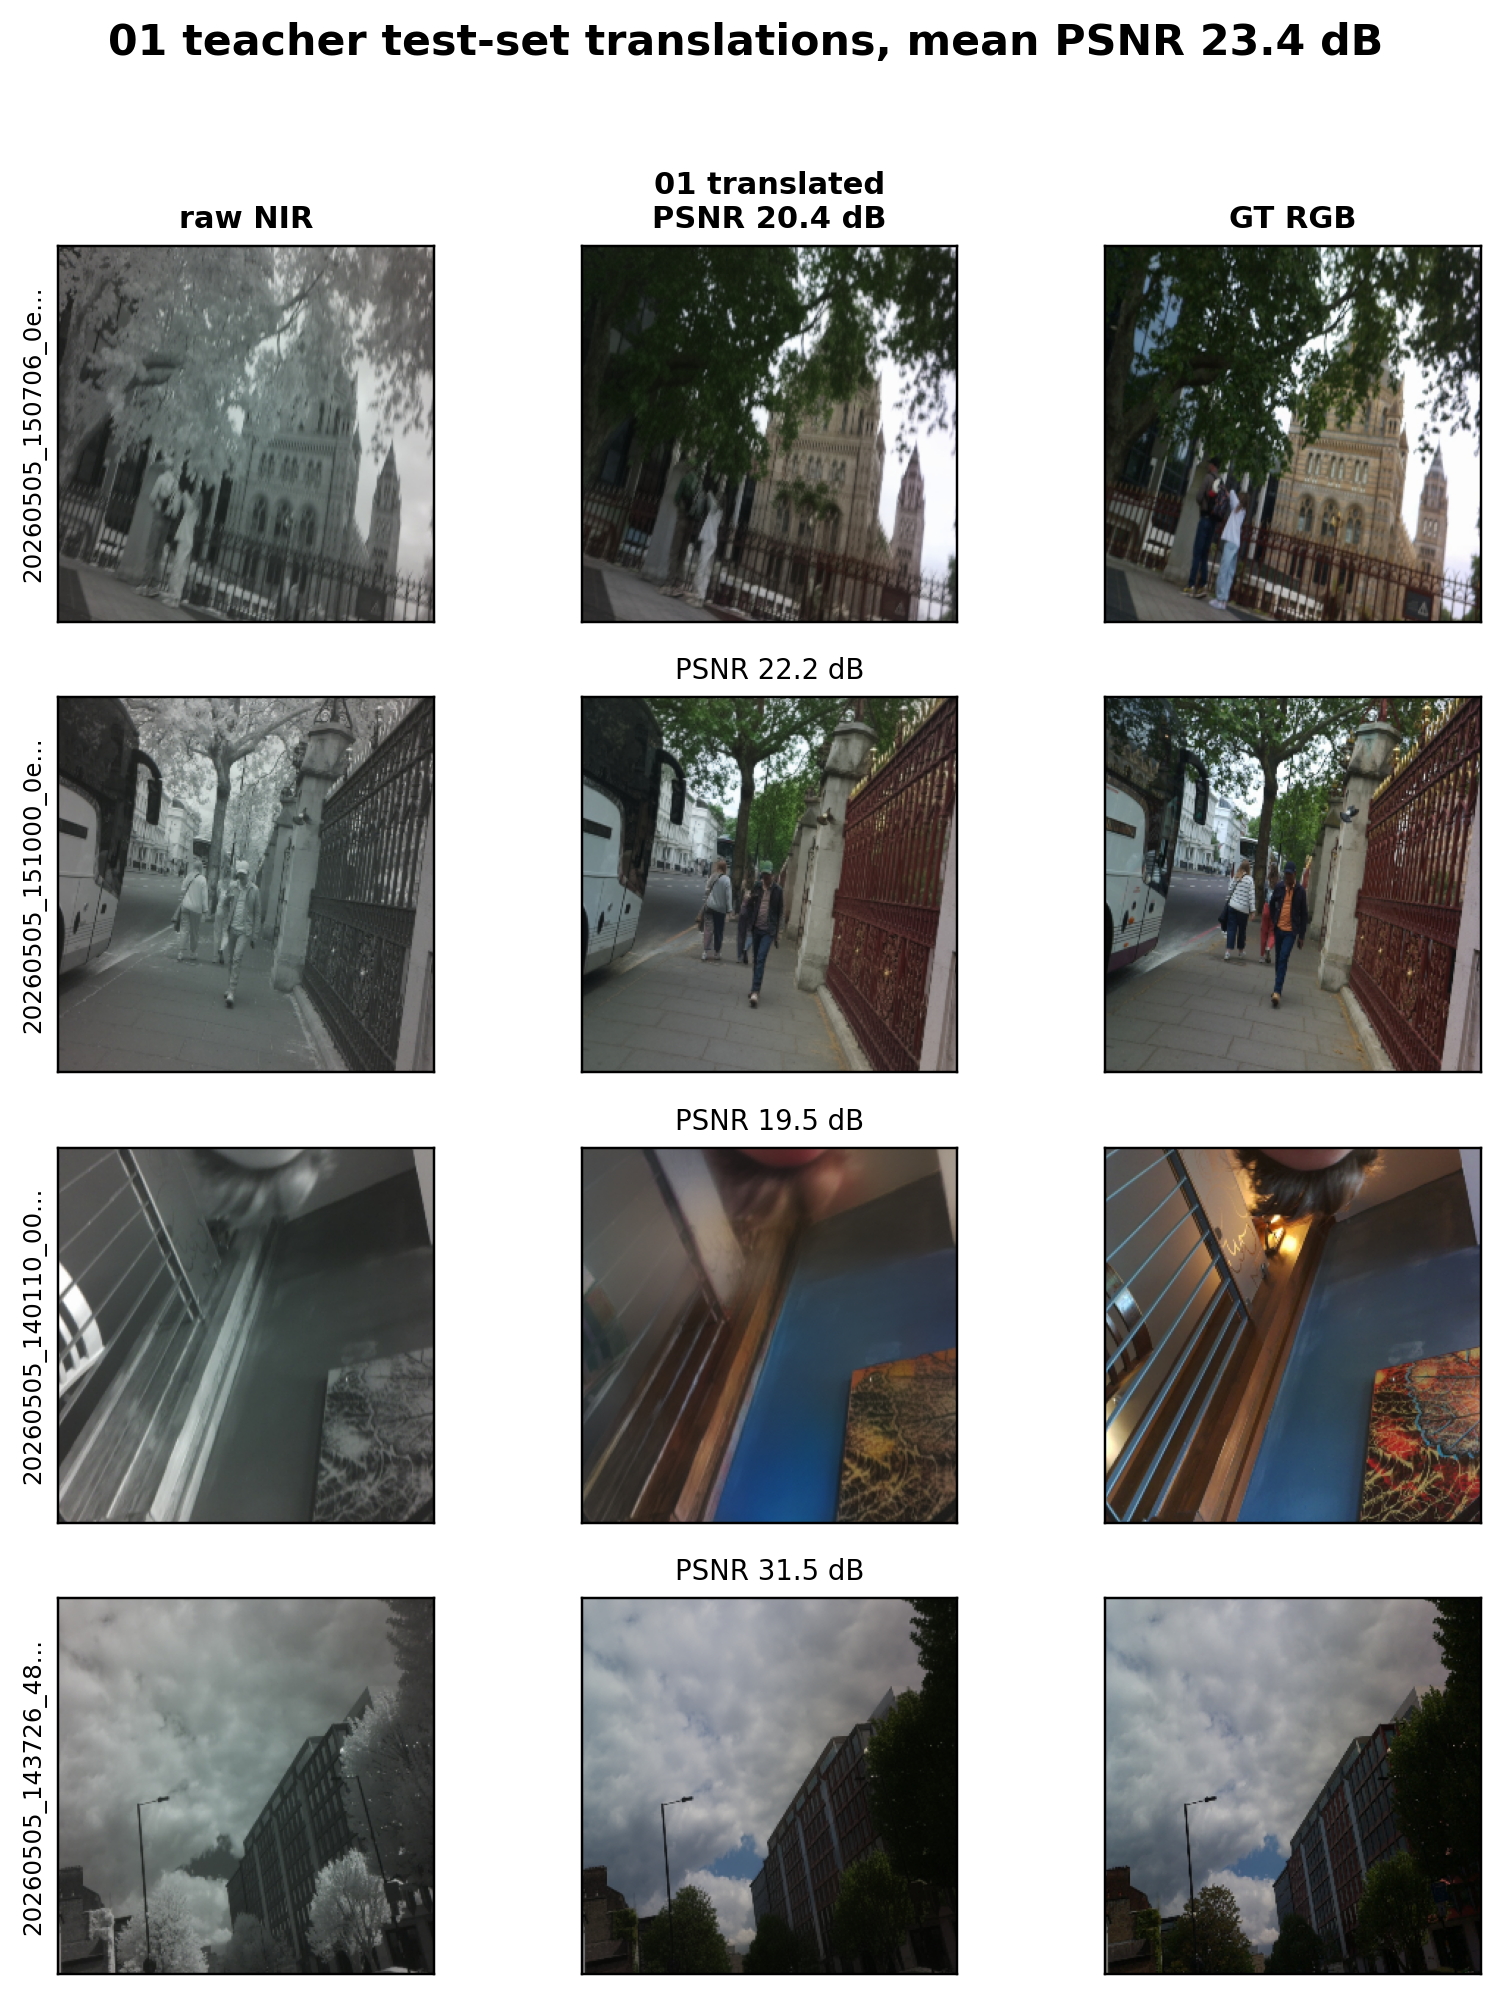
\includegraphics[width=0.82\textwidth]{figures/baseline_test_examples.png}
\end{center}

\textbf{Issues:} Person examples can look plausible globally while local people/skin/clothing are wrong or muted. Likely reasons: people are often a small part of the $256\times256$ training crop, skin colour is weakly determined from NIR, and the pixel/perceptual losses are dominated by large background areas.

\newpage
\section*{Attempts to improve downstream task performance}

\section*{Smart crop}

Smart crop is aimed at the person/MediaPipe failure mode. My idea is that when people are small in the frame, resizing the whole image to $256\times256$ leaves very little face/hand detail. This version uses cached MediaPipe boxes before resizing, so detected human/skin regions can be cropped first.

\begin{center}
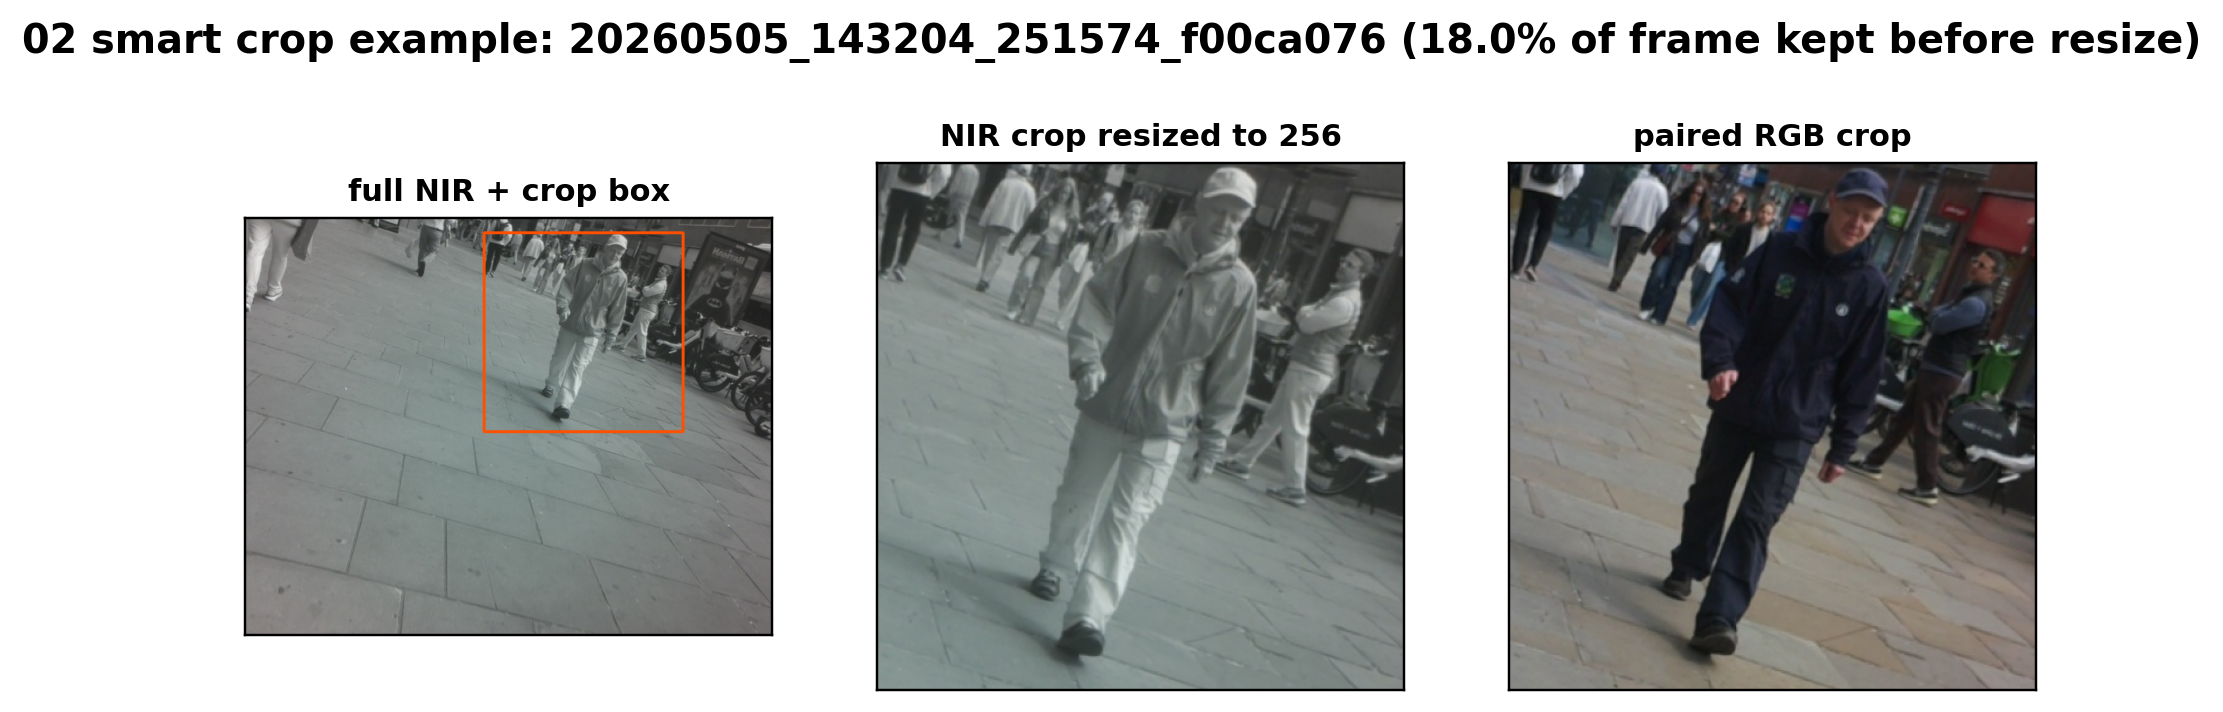
\includegraphics[width=0.98\textwidth]{figures/smartcrop_example.png}
\end{center}

\section*{Region L1 boost}

This targets the same issue without cropping. My idea is that faces/hands/people occupy too small a region, so normal L1 underweights them relative to pavement, sky, buildings, and trees. The model keeps the full frame but applies 5x L1 weight inside the cached MediaPipe region box.

\begin{center}
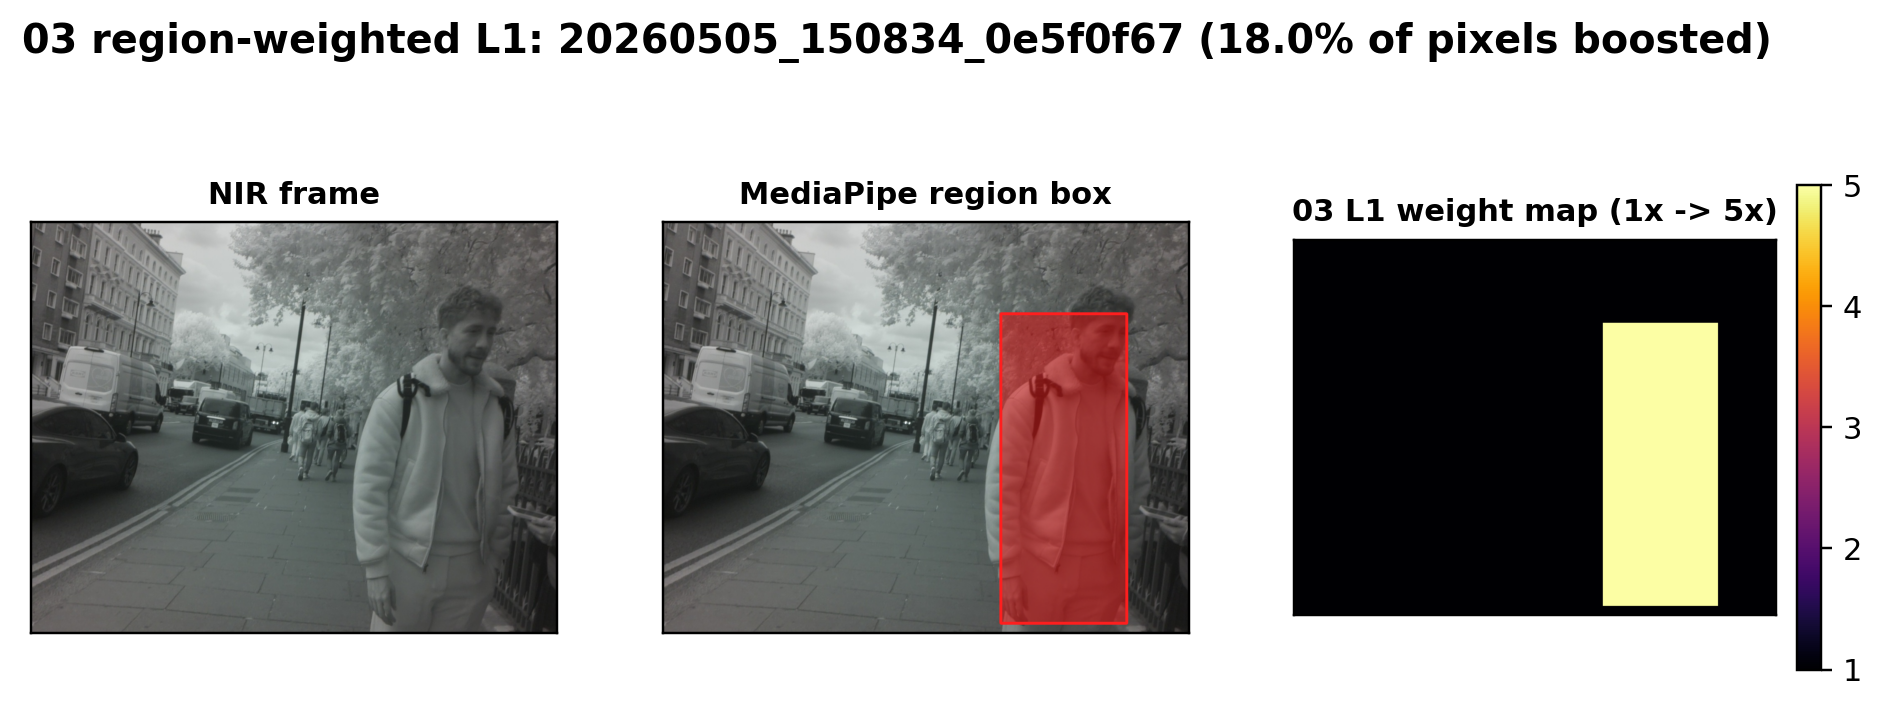
\includegraphics[width=0.98\textwidth]{figures/region_l1_overlay.png}
\end{center}

\newpage
\section*{NIR-gradient L1}

Some RGB colour is not inferable from flat NIR regions. My idea is that penalising those pixels equally can push the model toward average/desaturated colour, so this loss downweights L1 where local NIR variation is low.

\begin{center}
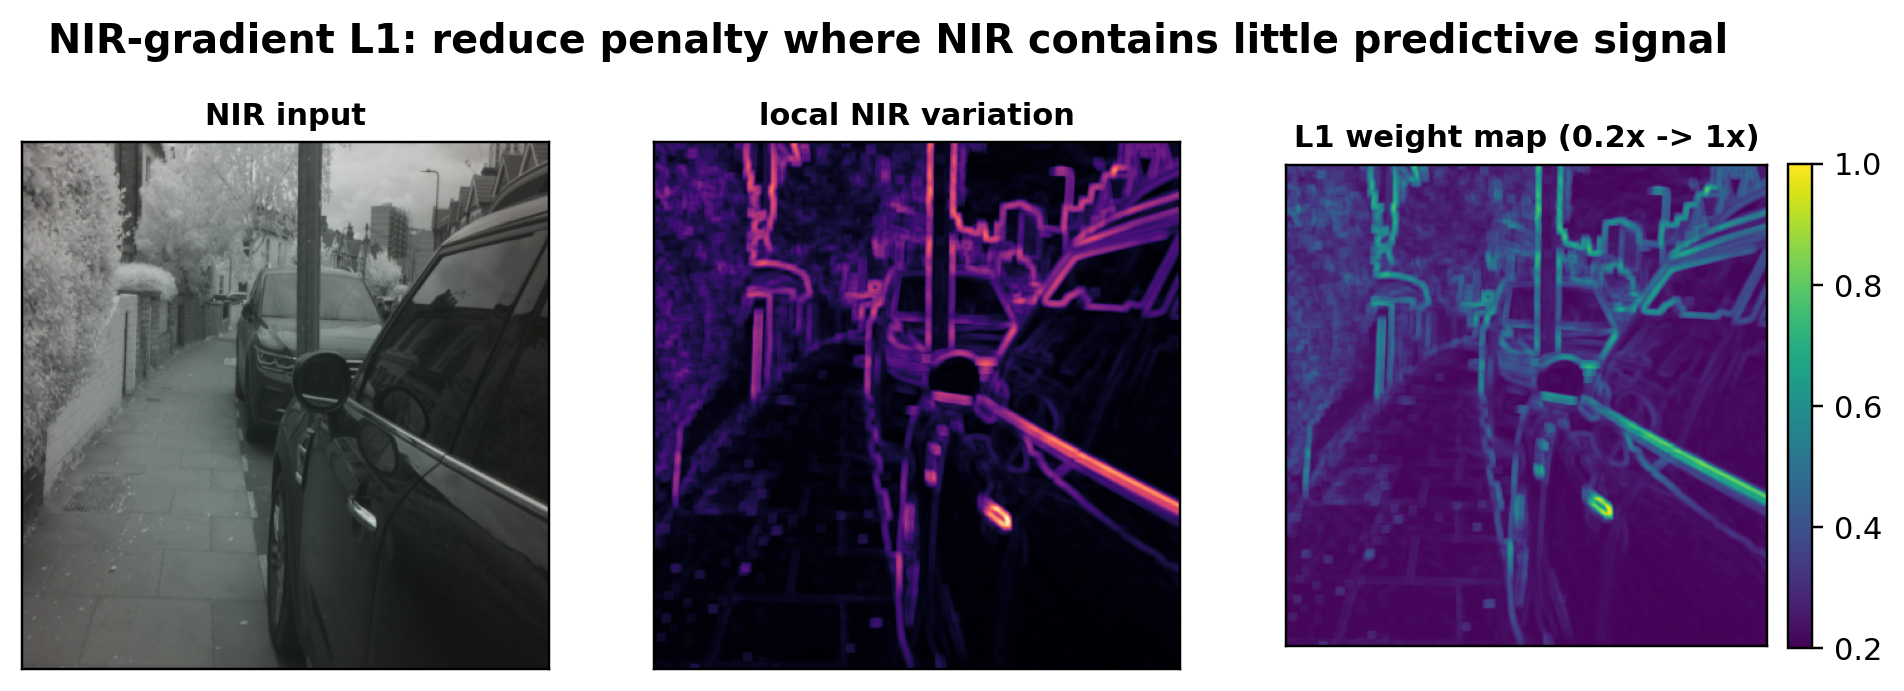
\includegraphics[width=0.98\textwidth]{figures/nir_gradient_l1.png}
\end{center}

\section*{Feature-map loss}

My plan is to train the same teacher setup, but add a task-facing feature loss from frozen RGB-trained models. The generated RGB and real RGB are both passed through ResNet50 and DeepLabV3-ResNet50, and the generator is pushed to match their early/mid activations. The goal is to make the output useful to downstream RGB models, not just visually close under pixel losses.

This setup uses the baseline-style full frame, $L_1$ weight reduced to 25, and a feature-map weight ramp from 0 to 50 over the first 5 epochs.

\begin{center}
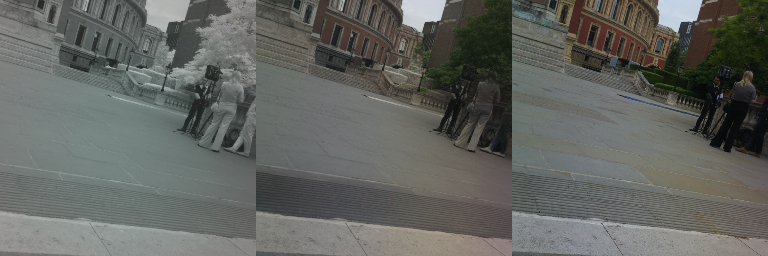
\includegraphics[width=0.88\textwidth]{figures/featuremap_step_00002000.png}
\end{center}

All these approaches are at various stages, and I will update you with the results of each of these experiments next time we meet.

\newpage
\section*{Training setup}

I am currently using Google Cloud Platform with the \$300 free credit for training. Runs are split across a mixture of L4 and A100 spot instances: A100s for the heavier teacher/distillation jobs, and L4s for cheaper ablations, inference checks, and export/deployment work. Because spot instances can be interrupted, the training scripts save regular checkpoints and random sample outputs.

\section*{Deployment: distil the best teacher}

The teacher is for quality. The deployment path is to distil into a smaller student and benchmark on edge hardware.

\begin{center}
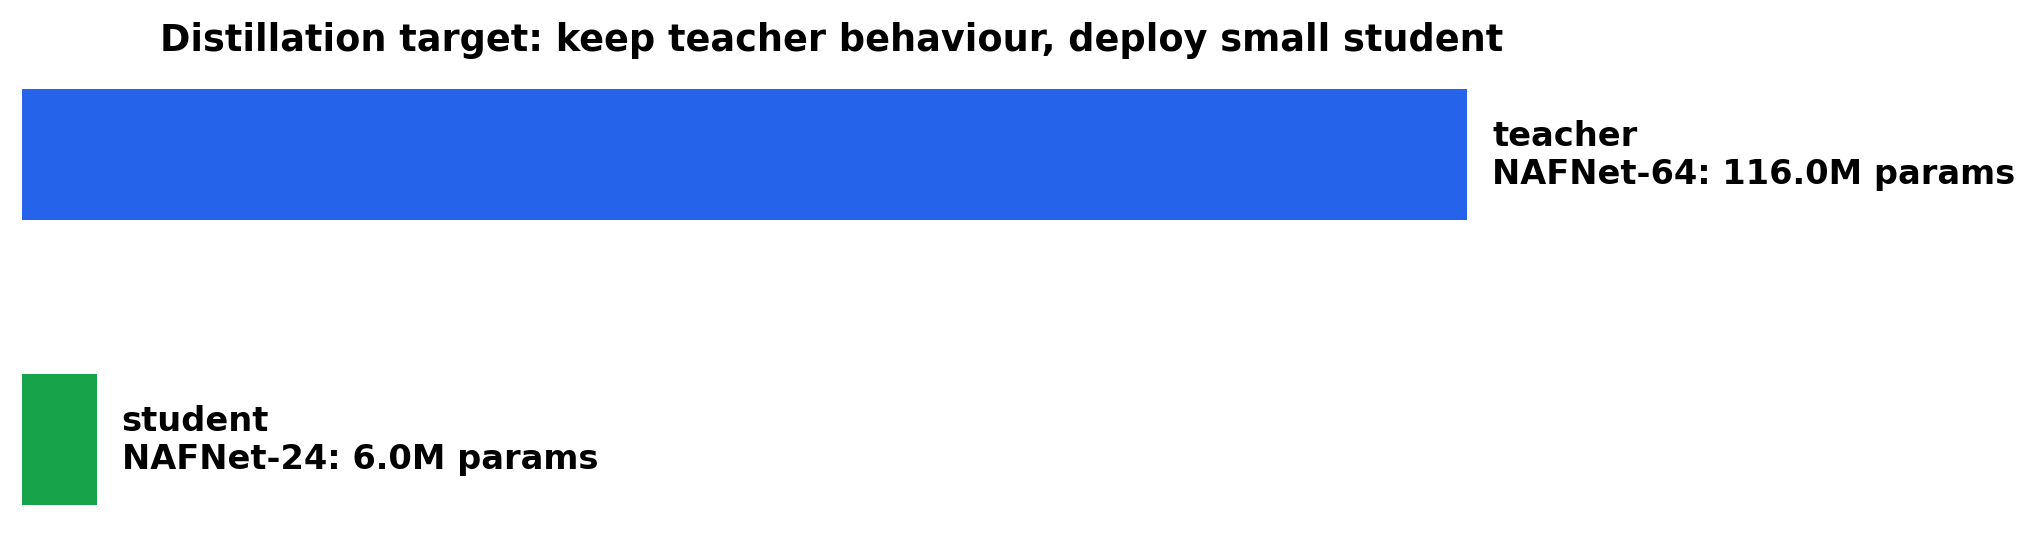
\includegraphics[width=0.86\textwidth]{figures/distillation_params.png}
\end{center}

\textbf{Distillation result.} The test distillation run worked: the 6.0M-parameter NAFNet-24 student is learning the teacher output while staying close to ground-truth RGB, and the model is small enough to run on a Raspberry Pi 5.

\begin{center}
\small
\begin{tabular}{lrrrr}
\toprule
Epoch & PSNR to GT & PSNR to teacher & SSIM to GT & SSIM to teacher \\
\midrule
53 & 22.56 dB & 27.02 dB & 0.802 & 0.941 \\
\bottomrule
\end{tabular}
\end{center}

\begin{center}
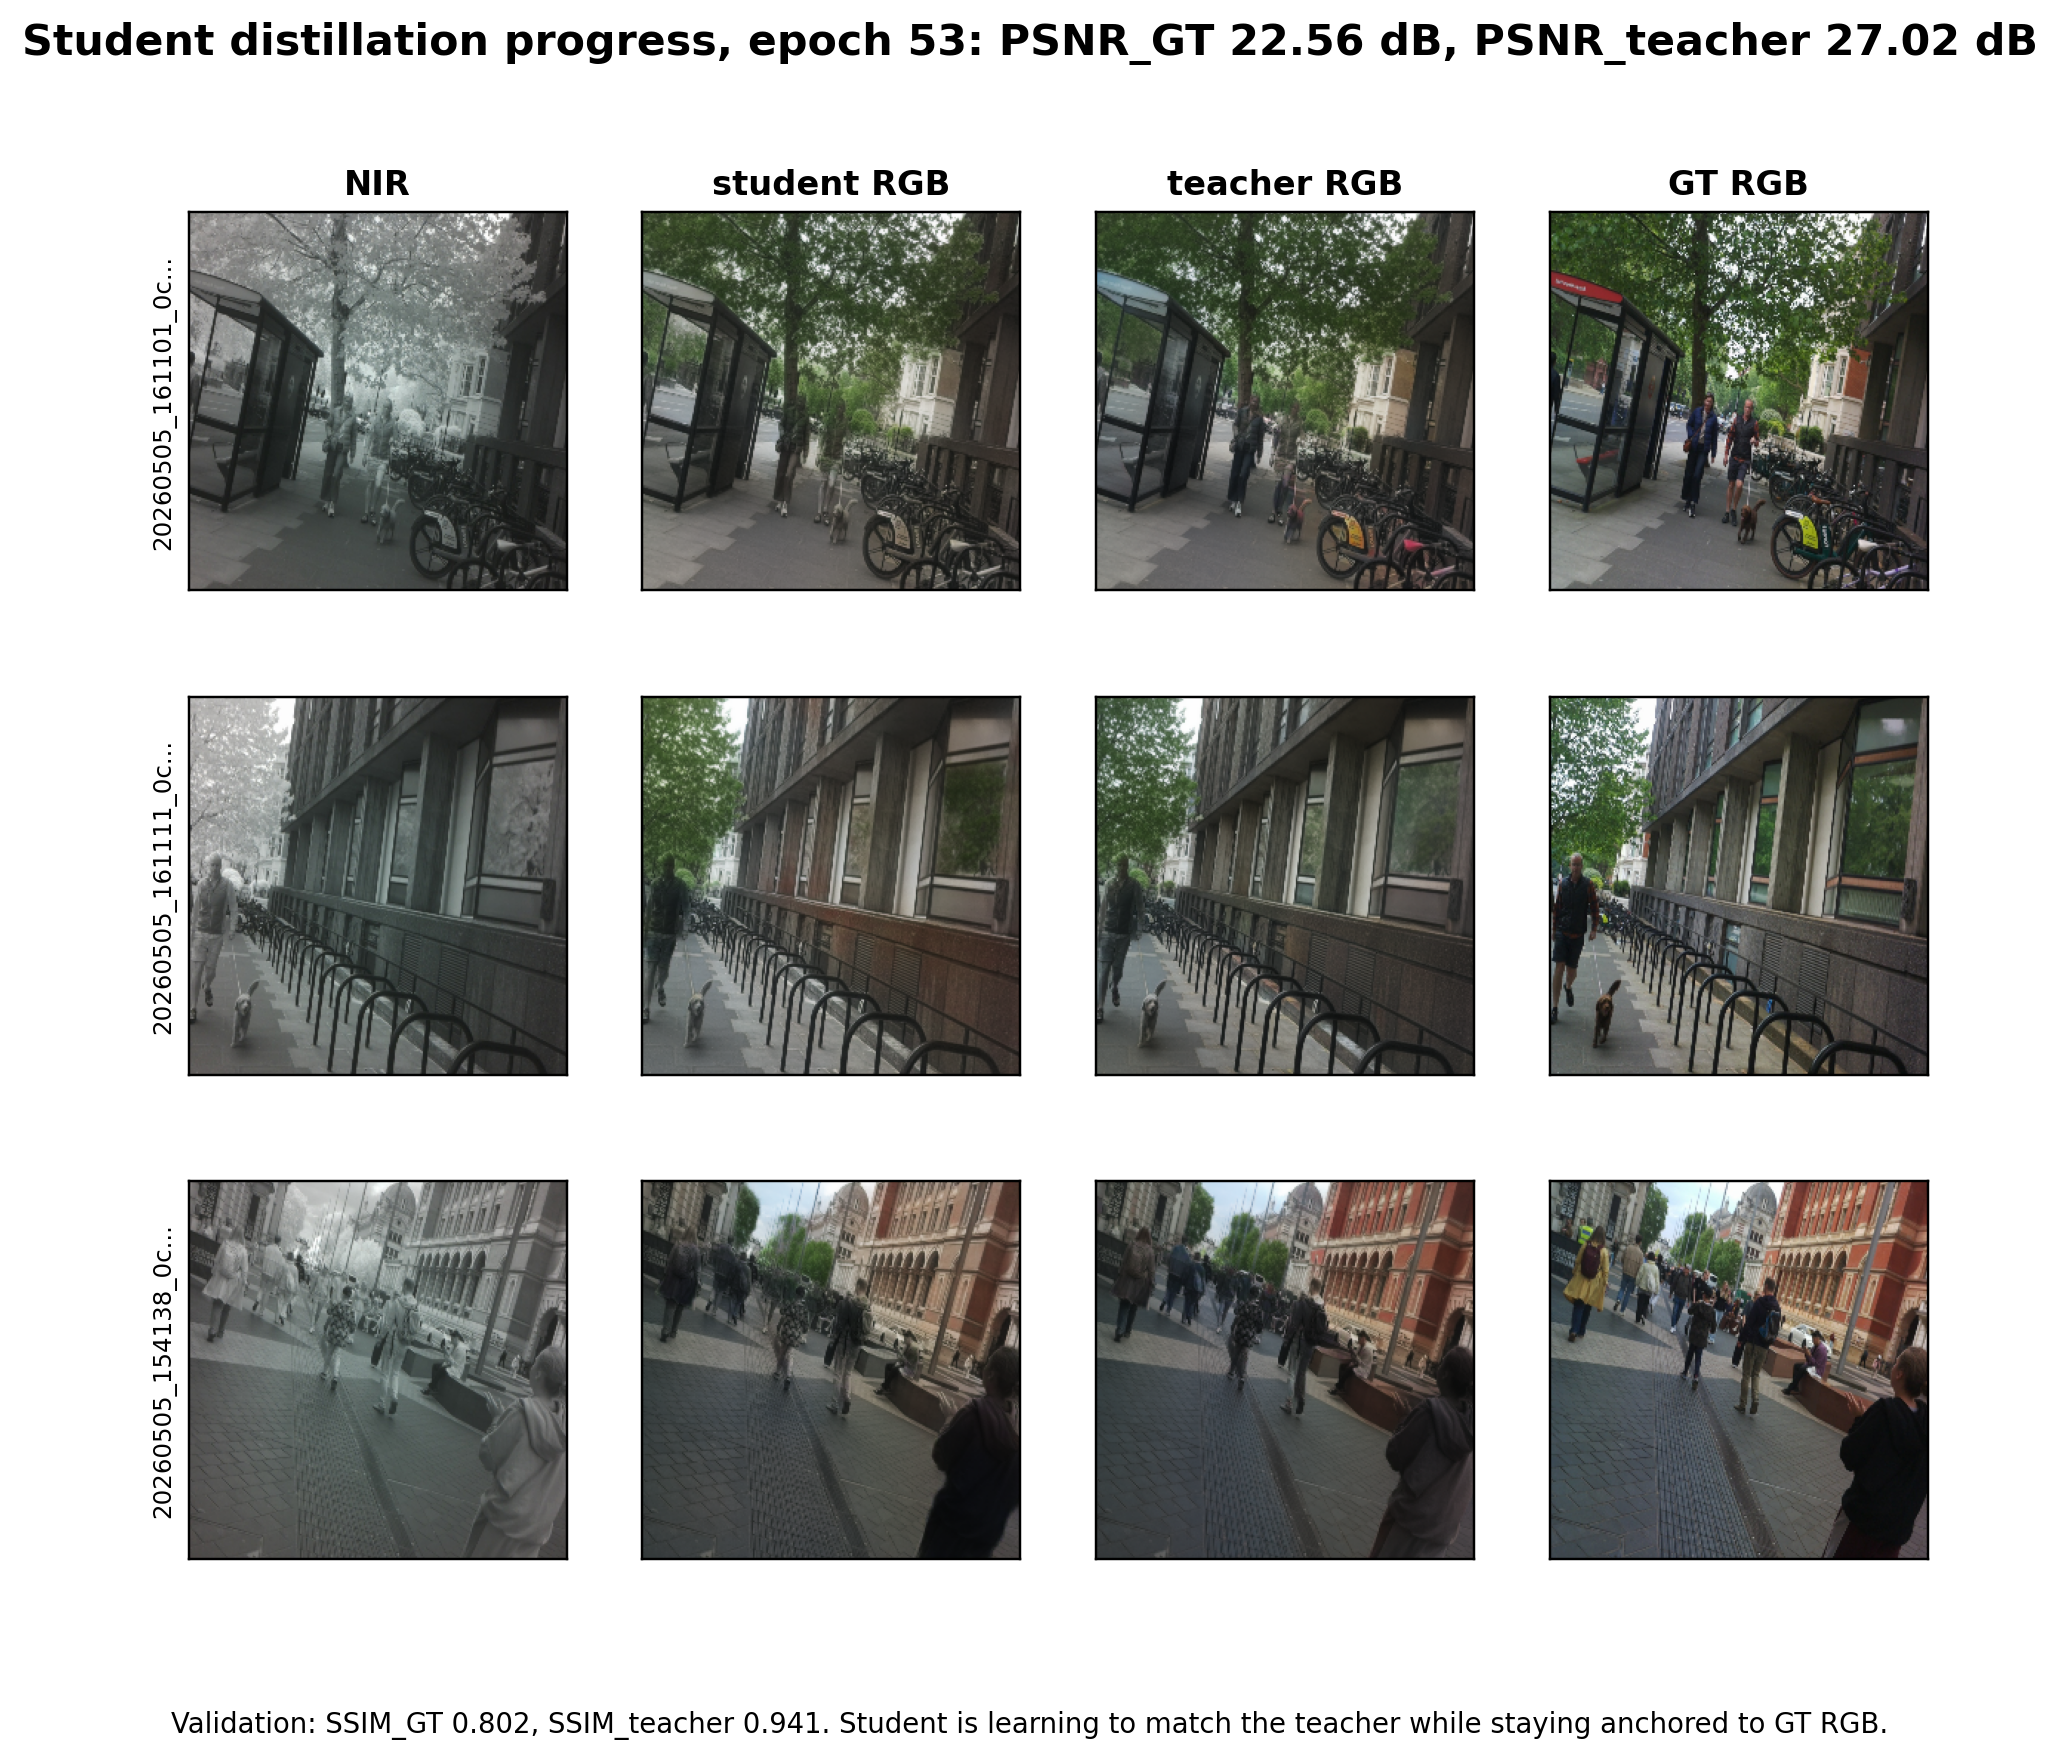
\includegraphics[width=0.98\textwidth]{figures/distillation_progress.png}
\end{center}

\end{document}
